\documentclass{acmart}
\usepackage[utf8]{inputenc}
\usepackage[spanish]{babel}
\usepackage{hyperref}

\title{Tarea 2 Bases de Datos Avanzadas}


\begin{document}

\maketitle

\tableofcontents

\section{Resumen}

\section{Introducción}

\section{H2}
\subsection{Arquitectura del DBMS}
\subsection{Tipo de almacenamiento utilizado}
\subsection{Representación en memoria}
\subsection{Mecanismos de compresión}
\subsection{Particionamiento}
\subsection{Operaciones DML}
\subsection{Buffer diferencial, proceso de mezcla}
\subsection{Reconstrucción de tuplas}
\subsection{Tipos de Joins}
\subsection{Logging / Recovery}
\subsection{Respaldos}
\subsection{Manejo de transacciones}
\subsection{Cold / Hot store}
\subsection{Manejo de datos históricos}
\newpage

\section{InMemory.NET}
Roberto Gervacio
\subsection{Arquitectura del DBMS}

Es un paquete autónomo donde se puede llamar directamente a la mayoría de las funciones. La idea de IRDB (InMemory.Net) es poder acceder a las ventajas de la tecnología en memoria directamente en el sistema y entorno ya existente. Los datos se comprimen y guardan en el disco como parte del proceso de importación. Estos archivos de datos comprimidos pueden ser leídos por el servidor IRDB. Extrae la información a través de ODBC, OLEDB o Dot Net Data Provider. Como se muestra en Fig \ref{irdb}.

\begin{figure}
	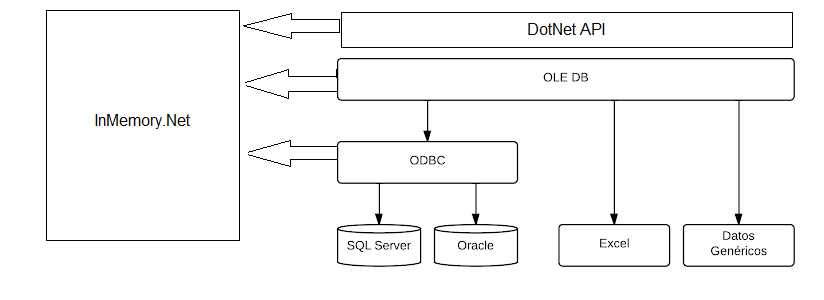
\includegraphics[width=\linewidth]{architecture_IRDB.png} % Figure image
	\caption{Arquitectura InMemory.NET} % Figure caption
	\label{irdb} % Label for referencing with \ref{irbd}
\end{figure}

\subsection{Tipo de almacenamiento utilizado}

Es una base de datos en memoria con almacenamiento columnar, diseñada para usar dentro del entorno Microsoft Dot Net. Aunque soporta la importación de tablas en modo no columnar, advierte funciona bien si solo hay unas pocas tablas involucradas. El modo NO COLUMNIZADO debe considerarse en este caso para estas tablas, ya que mantiene los datos en un estado sin columnas hasta que se emita el comando COLUMNIZE.

\subsection{Representación en memoria}

Para poder mantener tantos datos en la memoria como sea posible, los valores únicos dentro de cada columna se almacenan en una matriz de búsqueda. Otra matriz se utiliza como índice que corresponde con el valor real en la matriz de búsqueda.

\subsection{Mecanismos de compresión}

Cada valor se almacena una sola vez en lugar de varias veces. En el archivo físico comprimido, primero se guardan los valores únicos, seguidos del número requerido de bits utilizados para representarlo.

Cuando se carga en la memoria, se usan 8 bits (char) si el número de valores únicos es 255 o menos, 16 bits (ushort) si es 65535 o menos, de lo contrario, 32 bits (int).

\subsection{Particionamiento}

Al ser una base de datos con almacenamiento en columnas utiliza el particionamiento vertical. Aunque pude hacerlo horizontal, pero advierte disminuye el rendimiento en esas tablas.

\subsection{Operaciones DML}

\textbf{SELECT}: Es la piedra angular de cualquier consulta SQL. IRDB admite la sintaxis regular de selección de SQL.

\textbf{SELECT DISTINCT}: Es soportado pero está limitado internamente por el grupo por límites de cardinalidad.

\textbf{SELECT *}: Es soportad pero si se tiene columnas con caracteres no soportados, no se validarán y harán que la consulta se comporte mal. IRDB está diseñado para hacer consultas agregadas rápidamente. Las consultas no agregadas se ejecutarán y también continuará ejecutándose en su totalidad. Si selecciona una gran cantidad de registros las tablas con millones de registros no son un problema, pero si pasa una consulta que realiza un SELECT * desde una tabla con cientos de millones de registros, internamente va a través del proceso de creación de la tabla desde cero y columnizarla, posiblemente quedándose sin memoria.

\textbf{NOCACHE}: Como un refuerzo de rendimiento, IRDB crea tablas temporales cuando cree que las subconsultas podrían reutilizarse (por ejemplo, para JOIN anidados o donde se usan fechas dinámicas). La creación de estos archivos temporales se puede desactivar mediante la inclusión de NOCACHE.

\textbf{CACHE}: La creación las tablas temporales se puede desactivar mediante la inclusión de nocache = true en
archivo irdb.ini. La inclusión de la palabra clave CACHE en una declaración select, anula esta declaración por
usando caché.

\textbf{CASE STATEMENTS}: Suporta la siguiente estructura:
\begin{verbatim}
CASE WHEN logic_expression THEN SomeExpression
WHEN logic_expression2 THEN SomeExpression2
ELSE SomeOtherExpression END
\end{verbatim}

\textbf{COUNT}: Cuenta el número de filas de datos no nulos en la selección

\textbf{COUNT (DISTINCT)}: devuelve el número de valores distintos dentro de una tabla.

\textbf{SUM (DISTINCT)}: Cuando se le da un parámetro, realizará una suma única en esa columna. Si hay
valores duplicados solo se suman una vez. Con múltiples parámetros (que deben ser campos de la base de datos), encontrará los valores únicos, y suma la primera columna.

\textbf{OVER() / OVER (PARTITION BY )}: Permite que los valores que se devuelvan en función del resultado de una consulta secundaria dentro de una partición. Se utiliza principalmente con las funciones RANK () y DENSE\_RANK (). También se admiten SUM, MIN, MAX, ROW\_NUMBER.

\textbf{JOINS}: Revisar la sección de JOINS.

\textbf{GROUP BY, ORDER BY, HAVING}: Soporta las operaciones SQL.

\textbf{INTERSECT}: Devuelve las filas comunes entre dos instrucciones SELECT.

\textbf{EXCEPT}: Devuelve filas que están en una instrucción SELECT inicial, pero no en una consulta secundaria.

\textbf{UPDATE}: La actualización en IRDB funciona de manera similar a otras bases de datos como SQL Server. Si está consultando un actualiza en la versión actual en memoria solamente. Los cambios no se conservan en el disco.

\textbf{DELETE}: Hay soporte de eliminación momenatnea. Si se emite el comando Delete, se elimina solo en la versión actual en memoria. Los cambios no son conservados en disco.

\subsection{Buffer diferencial, proceso de mezcla}

No hay información en la documentación referente a este tópico.

\subsection{Reconstrucción de tuplas}

Lo hace mediante ordenamiento natural en todas las columnas en ambas tablas, luego haciendo una fusión entre ellas para encontrar las filas comunes.

Implementa un algoritmo de clasificación al ordenar tablas grandes con grandes cantidades de columnas. Anteriormente utilizaba BigIntegers para clasificación. Sin embargo, era muy lento al ordenar grandes cantidades de columnas. Ahora sus algoritmos mejorados utilizan estructuras de longitudes de varios tamaños, y generan dinámicamente código y compilaciones para hacer la configuración de clasificación.

\subsection{Tipos de Joins}

Actualmente IRDB admite INNER y LEFT y CROSS, RIGHT JOINS y Full Joins. Se ejecutan mejor si tiene la tabla con la cardinalidad más alta primero, uniéndose contra las tablas con granularidad decreciente. Todos los joins son conducidas por la primera tabla que se asumen es la tabla principal. Soporta joins de hasta 50 dimensiones. Las consultas deben diseñarse sin bucles de unión y unirse de tal manera que las uniones fluyan desde la primera tabla o las tablas de nivel superior. Expresiones de los campos que involucran la misma tabla ahora son compatibles. Actualmente constantes por sí mismas no son compatibles.

\subsection{Logging / Recovery}

Almacena un registro lógico en el directorio principal. Proporciona un registro de los queriess que se ejecutan y un desglose de los principales momentos de ejecución que se realizaron en la consulta.

\subsection{Respaldos}

La forma de obtener infomación es a través de la importación de algun ODBC u OLEDB. Por lo que el único respaldo posible es mediante la exportación desde IRDB como parte de un script IRDBIMPORT. Para esto las tablas deben ser importado dentro de la secuencia de comandos antes de exportar.

\begin{verbatim}
--import statement

SAVE TABLA <tableName> TO CSV <nombre de archivo>
\end{verbatim}

\subsection{Manejo de transacciones}

No cuenta con el soporte para transacciones.

\subsection{Cold / Hot store}

Se basa en hot storage. Ya que todo el tiempo la infomación se encuentra en memoria y esta diseñada para cargas de trabajo con muchas transacciones.

\subsection{Manejo de datos históricos}

No cuenta el soporte para datos históricos.

\newpage

\section{MySQL NDB Cluster}
Yann Le Lorier Bárcena
El DBMS de MySQL NDB Cluster es un sistema de administración de alta redundancia que está pensado para la computación distribuida (Oracle, s.f.)
\subsection{Arquitectura del DBMS}
La arquitectura del DBMS es la famosa three-tier architecture, separando en capas independientes los elementos entre el usuario y los datos en la BD.\\
Por otro lado, este DBMS está pensado como un sistema \textit{shared-nothing}, es decir que cada componente debe de tener su propio disco y memoria, por lo que la memoria compartida no es recomendable para este administrador.
\subsection{Tipo de almacenamiento utilizado}
\subsection{Representación en memoria}
\subsection{Mecanismos de compresión}
De acuerdo con la información extraída de la documentación sobre las definiciones de la creación del Cluster (\cite{mysqlcomp}), dentro de la base de datos, existe un conjunto de variables que permiten comprimir:
\begin{itemize}
    \item los respaldos, y reducir el espacio utilizado en el disco, de 50\% o más. Se trata de una compresión que es equivalente al \textit{gzip--fast}. La elección entre tener o no activados los backups puede ser realizada para nodos individuales, o para todos los nodos.
    \item Se pueden también comprimir archivos de los \textit{local checkpoint files}, que utilizan una compresión que es de igual manera, equivalente al \textit{gzip--fast}
\end{itemize}


\subsection{Particionamiento}
En MySQL NDB Cluster, el particionamiento se conoce como \say{Replicas}. Se dividen por los Clusters, que dividen la información a guardar, dependiendo de la partición que se le haya asignado. Todo este proceso es manejado automáticamente por el DBMS.\\
Es posible definir el particionamiento al nivel usuario, el NDBCLUSTER, que es usualmente definido automáticamente.\\
La \textit{Replicas} son copias de una partición del cluster. Cada nodo en un grupo de nodos contiene una réplica. Se trata de una relación 1 a n entre la réplica y el nodo, ya que por cada nodo, normalmente existen muchas réplicas, podemos observar un ejemplo en la imagen \ref{dosnodos}.

\begin{figure}
    \centering
    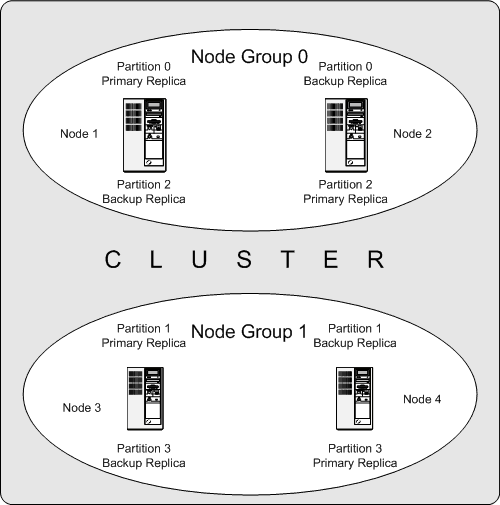
\includegraphics[width=0.4\linewidth]{replicas.png}
    \caption{Un Cluster con dos grupos de nodos}
    \label{dosnodos}
\end{figure}

\subsection{Operaciones DML}

\subsection{Buffer diferencial, proceso de mezcla}
NDB usa uno o más buffers de memoria para los eventos de los nodos que contienen la información. Para cada objeto NDB, existe un buffer que registra la información de los eventos que van sucediendo a nivel tabla, por lo que existe otro buffer que va registrando la información del esquema (Oracle, s.f., \cite{mysqlbuff}).\\
Estos buffers van imprimiendo su estado en el cluster log.
\subsection{Reconstrucción de tuplas}
\subsection{Tipos de Joins}
\subsection{Logging / Recovery}
\subsection{Respaldos}
Los respaldos de esta DBMS están basados en tres principales partes:
\begin{itemize}
    \item Metadata: Nombres y definiciones de todas las tablas de la base de datos
    \item Registros de tablas: la infomación que está guardada dentro de las tablas al momento de realizar el respaldo
    \item Registro de las transacciones: Se trata de un registro secuencial que tiene las 'instrucciones' para obtener la base de datos al momento del respaldo.
\end{itemize}
(Oracle, s.f. \cite{mysqlbackups})\\
Todos los nodos realizan cada uno el respaldo con las tres partes mencionadas anteriormente, las cuales se guardan en tres archivos en el disco del nodo:
\begin{itemize}
    \item \textit{<backup.id>.<node.id>.ctl} Toda la información de control y la metadata mencionada anteriormente
    \item \textit{<backup.id>.<node.id>.data} Un archivo que contiene toda la información con la que la tabla está rellenada. La información está fragmentada, dependiendo del nodo en cuestión, guardando información parcial de alguna tabla.
    \item \textit{<backup.id>.<node.id>.log} Un registro de transacciones a las que se les realizaron el \textit{commit}. De igual forma que el archivo de data, son diferentes registros por que la información está fragmentada.
\end{itemize}
\subsection{Manejo de transacciones}
Como lo dice su nombre, MySQL NDB Cluster, es un DBMS que está previsto para información fragmentada, en nodos de computación con su propia memoria y su propio disco.
En cada cluster de la base de datos, existe una tabla en particular que se llama \textit{cluster\_transactions} que es una tabla que muestra todas las transacciones que están ocurriendo en un cluster.\\
A continuación se describe la tabla \textit{cluster\_transactions} por columna:

\begin{center}
    \begin{tabular}{|c|c|}
        \hline
        node\_id & id del nodo que es el coordenador de la transacción \\
        \hline
        block\_instance & la instancia del bloque realizando la transacción \\
        \hline
        transid & id de la transacción \\
        \hline
        state & estado de operación\\
        \hline
        count\_operations & número de operaciones con llave primaria en la transacción \\
        \hline
        outstanding\_operations & operaciones que siguen siendo ejecutadas en los bloques locales de administración\\
        \hline
        inactive\_seconds & tiempo que ha transcurrido esperando al API \\
        \hline
        client\_node\_id & Id del nodo del cliente\\
        \hline
        client\_block\_ref & referencia del bloque del cliente\\
        \hline
    \end{tabular}
    \captionof{table}{descripción por columna de la tabla cluster\_transactions}
\end{center}

Analizando los inconvenientes del manejo de transacciones, podemos notar ciertos aspectos:
\begin{itemize}
    \item Soporte de sólamente las transacciones a las que se les hicieron "commit", por lo que no se pueden ver las transacciones sin este proceso.
    \item Procesamiento intensivo de las transacciones por que cada una tiene que tener forzosamente la fase de \say{commit}
    \item No existen las transacciones parciales, ya que si se realiza un \say{rollback}, descarta desde el principio de la transacción, a diferencia de InnoDB, el cual permite el \say{rollback} de \say{statements} individuales.
\end{itemize}
(Oracle, s.f., \cite{mysqllimittrans})
\subsection{Cold / Hot store}
Mientras que en la documentación no existe una sección dedicada al Hot \& Cold storage, se menciona en la sección de backup troubleshooting. En esta sección habla que la recuperación de datos del backup es \say{hot} pero no lo es realmente en su totalidad, ya que explica que no existe soporte para lecturas repetidas (\textit{repeatable reads}), es decir que el DBMS no puede garantizar durante el proceso de respaldo que si intentamos leer la información nuevamente obtendremos el mismo resultado, por lo tanto existe información que es inconsistente durante este momento. (Oracle, s.f., \cite{mysqlhot})

\subsection{Manejo de datos históricos}

\newpage

\section{Raima}
Isaac Harari Maasri
\subsection{Arquitectura del DBMS}
\subsection{Tipo de almacenamiento utilizado}
\subsection{Representación en memoria}
\subsection{Mecanismos de compresión}
\subsection{Particionamiento}
\subsection{Operaciones DML}
\subsection{Buffer diferencial, proceso de mezcla}
\subsection{Reconstrucción de tuplas}
\subsection{Tipos de Joins}
\subsection{Logging / Recovery}
\subsection{Respaldos}
\subsection{Manejo de transacciones}
\subsection{Cold / Hot store}
\subsection{Manejo de datos históricos}

\newpage

\section{Comparación entre DBMS}

\section{Conclusiones}

\begin{thebibliography}{99}
	\bibitem{mysqlbackups} Oracle. (n.d.). MySQL NDB Cluster Online Backup. Retrieved March 21, 2020, from https://dev.mysql.com/doc/mysql-cluster-excerpt/8.0/en/mysql-cluster-backup.html
	\bibitem{mysqltransactions} Oracle. (n.d.). MySQL NDB Cluster The ndbinfo cluster\_transactions Table. Retrieved March 21, 2020, from https://dev.mysql.com/doc/mysql-cluster-excerpt/8.0/en/mysql-cluster-ndbinfo-cluster-transactions.html
	\bibitem{mysqlhot} Oracle. (n.d.). MySQL NDB Cluster NDB Cluster Backup Troubleshooting. Retrieved March 21, 2020, from https://dev.mysql.com/doc/mysql-cluster-excerpt/8.0/en/mysql-cluster-backup-troubleshooting.html
	\bibitem{mysqllimittrans} Oracle. (n.d.). MySQL NDB Cluster Limits Relating to Transaction Handling in NDB Cluster. Retrieved March 21, 2020, from https://dev.mysql.com/doc/mysql-cluster-excerpt/5.7/en/mysql-cluster-limitations-transactions.html
	\bibitem{mysqlcomp} Oracle. (n.d.). MySQL NDB Cluster 8.0 :: 5.3.6 Defining NDB Cluster Data Nodes. Retrieved March 21, 2020, from https://dev.mysql.com/doc/mysql-cluster-excerpt/8.0/en/mysql-cluster-ndbd-definition.html
	\bibitem{mysqlpart} Oracle. (n.d.). MySQL 5.7 Reference Manual :: 21.1.2 NDB Cluster Nodes, Node Groups, Replicas, and Partitions. Retrieved March 21, 2020, from https://dev.mysql.com/doc/refman/5.7/en/mysql-cluster-nodes-groups.html
	\bibitem{mysqlbuff} Oracle. (n.d.). MySQL NDB Cluster 8.0 :: 7.7.3 Event Buffer Reporting in the Cluster Log. Retrieved March 22, 2020, from https://dev.mysql.com/doc/mysql-cluster-excerpt/8.0/en/mysql-cluster-logs-event-buffer.html
	\bibitem{inmemorynet} 
	In-Memory.NET,
	\\\texttt{https://inmemory.net/blog/}

\end{thebibliography}

\end{document}